\documentclass{article}
\usepackage[spanish]{babel}   
\usepackage[numbers,sort&compress]{natbib}
\usepackage{float}
\usepackage{listings}
\usepackage{graphicx} 	% Nos permite importar imagenes 
\usepackage{subcaption}
\usepackage[left=3cm,right=3cm,top=3cm,bottom=3cm]{geometry}

%-------------------------- Por si se romple la URL --------------------------
\usepackage[hyphens]{url}
\usepackage[hidelinks]{hyperref}
\hypersetup{breaklinks=true}	
\urlstyle{same}
\usepackage{cite}
%-------------------------- Por si se romple la URL --------------------------

\title{Reporte Tarea 6}
\author{Victor Alejandro Oviedo Martínez}



\begin{document}
\maketitle
\hrule

\section{Introduccón}\label{intro}
Para esta sexta tarea\citep{DRA.P6} se ha estudiado el tema sistema multiagente, específicamente para simulación epidemiológica. En esta simulación cada agente tendrá tres diferentes estados de salud, \textbf{S}usceptible, \textbf{I}nfectado o \textbf{R}ecuperado. Como parámetros de simulación se deberá especificar; área de simulación $(l  {\times}  l)$, número de agentes $(n)$, probabilidad de infección al inicio $(Pi)$, probabilidad de recuperación $(Pr)$, distancia segura $(r)$, y velocidad $(v)$. Una vez conocidos los parámetros, debemos entender que cada agente tendrá  parámetros propios como; posición $(x,y)$, velocidad y dirección $({\Delta}x,{\Delta}y)$, y estado $(S, I)$ tomando en cuenta que este estado dependerá de $Pi$, es importante mencionar que el estado $R$ se podrá obtener una vez pasado el estado $I$, una vez que el estado del agente sea $R$, este contará con inmunidad permanente. Una vez definidos los parámetros de cada uno de los agentes se podrá iniciar la simulación. Ya en la simulación, para cambiar de estado $S$ a estado $I$ se evaluará con la probabilidad de contagio $(Pc)$, la cual depende de la distancia euclideana entre dos agentes $d(i,j)$ dado por:\\

\begin{equation}
Pc=\left\lbrace\begin{array}{c} 0,~~~~~~~~~~si~d(i,j) \geq r, \\ \frac{r - d}{r},~~~~~~ en~otro~caso, \end{array}\right.
\end{equation}


~~~~~~~~~~~~~~~~~~~~~~~~~~~~~~~~~~~~~~~~donde $r$ es un umbral.\\

De esta forma se podrá simular la pandemia dependiendo de los valores que se le asignen a las variables. 




 

\section{Desarrollo}

Para esta sexta tarea se ha planteado el siguiente problema: Vacuna con probabilidad $Pv$ a los agentes al momento de crearlos de tal forma que están desde el inicio en el estado $R$ y ya no podrán contagiarse ni propagar la infección. Estudia el efecto estadístico del valor $Pv$ de en (de cero a uno en pasos de 0.1) el porcentaje máximo de infectados durante la simulación y el momento (iteración) en el cual se alcanza ese máximo.\\

Para el desarrollo de esta tarea se a utilizado el código ejemplo proporcionado por \citet{DRA.Code}, el cual tiene el propósito de simular pandemias hasta un número determinado de repeticiones o si la cantidad de infectados es cero. Este código será tomando como base para ser modificado y entregar las características de esta tarea.\\

La edición de este código empieza generando un vector $Pv$ el cual tendrá los diferentes valores para la probabilidad de vacuna $(Pv)$ 

\begin{lstlisting}[language=Python]

pv = [d for d in np.arange(0, 1, 0.1)]

 \end{lstlisting}

Luego, se agregó un ciclo \texttt{for} el cual será el responsable de ejecutar $Pv$ veces la simulación, a su vez se ha editado la creación del DataFrame con el fin de agregar la probabilidad de vacuna $(Pv)$.
 
 \begin{lstlisting}[language=Python]
 
for pv in pv:
    print("-----------------", pv, "-----------------")

    agentes =  pd.DataFrame()
    agentes['x'] = [uniform(0, l) for i in range(n)]
    agentes['y'] = [uniform(0, l) for i in range(n)]
    agentes['dx'] = [uniform(-v, v) for i in range(n)]
    agentes['dy'] = [uniform(-v, v) for i in range(n)]

    for i in range(n):
        agentes.at[i, 'estado'] = 'S'
        if random() < pi:
            agentes.at[i, 'estado'] = 'I'
        else:
            if random() < pv:
                agentes.at[i, 'estado'] = 'R'
                
 \end{lstlisting}

Después de la edición del DataFrame el código es prácticamente el mismo hasta llegar a la parte final del bucle \texttt{for}, en donde se ha agregado el calculo para determinar el contagio máximo y el primer momento en el que este sucede. Una vez determinados estos dos valores serán impresos en terminal.

\begin{lstlisting}[language=Python]
    cont = 0
    max_contagio = max(epidemia)
    for x in range(len(epidemia)):
        if epidemia[x] == max_contagio:
            cont = cont + 1
            if cont == 1:
                momento_max_contagio = x

    print("Maximo contagio:", max_contagio)
    print("El maximo contagio se tuvo en la iteracion:", 
    momento_max_contagio)
 \end{lstlisting}

Antes de poder concluir tendremos que transformar los datos de las pandemias en en función del porcentaje máximo de cada pandemia.

\begin{lstlisting}[language=Python]
    conjuntox_epidemias.append(epidemia)
    conjuntoy = [100 * e / n for e in epidemia]
    conjuntoy_epidemias. append(conjuntoy)
 \end{lstlisting}

Finalmente, una vez simuladas todas epidemias con diferente $Pv$ se procede a generar la grafica con las simulaciones.\\

\begin{lstlisting}[language=Python]
label=['0.0','0.1','0.2','0.3','0.4','0.5','0.6','0.7','0.8','0.9']
for a in range(len(conjuntox_epidemias)):
    plt.plot(range(len(conjuntox_epidemias[a])),conjuntoy_epidemias[a], label=label[a])
plt.xlabel('Tiempo')
plt.ylabel('Porcentaje de infectados (%)')
plt.legend()
plt.show()
plt.close()
 \end{lstlisting}

Para el desarrollo de esta tarea se utilizó la pagina \citep{DRA.Code}.


\section{Conclusión}

Una vez ejecutado el programa se ha generado la figura \ref{fig:cuadro.1}, de la misma forma tendremos los datos  de contagio máximo y el primer momento en el que este sucede en la terminal, esta información podrá ser observada en el archivo \texttt{Datos.txt}, ó  en el cuadro \ref{fig:cuadro1}.


\begin{table}[H]
\centering
\caption{Datos resultados de la simulación.}
\label{fig:cuadro1}
\begin{tabular}{|c|c|c|}
\hline
$Pv$ & Contagio máximo & Tiempo de contagio máximo\\
\hline
0.0& 74 & 21\\
0.1& 68 & 39\\
0.2& 54 & 34\\
0.3& 41 & 29\\
0.4& 26 & 37\\
0.5& 30 & 40\\
0.6& 31 & 47\\
0.7& 22 & 63\\
0.8& 14 & 48\\
0.9& 1 & 0\\

\hline
\end{tabular}
\end{table}



\begin{figure}[H]
\begin{center}
	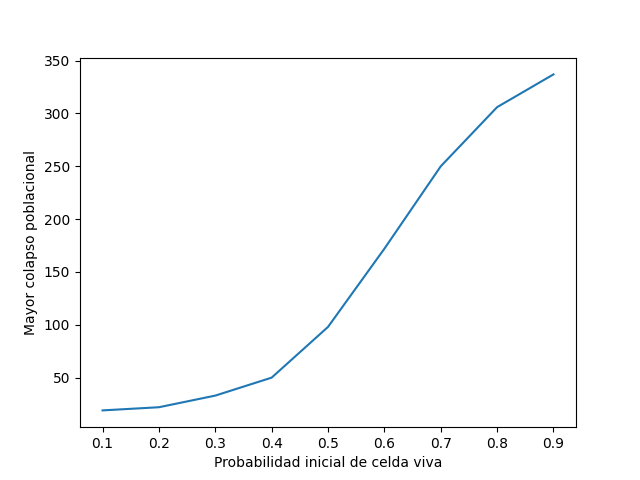
\includegraphics[height=3in]{/Users/victor/Desktop/Figure_1.png}
	\caption{ Resultados de la simulación hasta 200 repeticiones con variación en la probabilidad de vacunación  $(Pv)$.}
	\label{fig:cuadro.1}
\end{center}
\end{figure}

Como conclusión, se puede observar en la  figura \ref{fig:cuadro.1} como mientras mas alto sea el porcentaje de vacunación $(Pv)$ menor será el pico de contagio máximo y la pendiente de contagios será menos pronunciada. 

%-------------------------- Por si se rompe la URL --------------------------
\Urlmuskip=0mu plus 1mu\relax
%-------------------------- Por si se rompe la URL --------------------------
\bibliography{ref.Tarea6.bib}
\bibliographystyle{plainnat}

\end{document}